% 	%Template by Mark Jervelund - 2015 - mjerv15@student.sdu.dk

\documentclass[a4paper,10pt,titlepage]{report}

\usepackage[utf8]{inputenc}
\usepackage[T1]{fontenc}
\usepackage[english]{babel}
\usepackage{amssymb}
\usepackage{amsmath}
\usepackage{amsthm}
\usepackage{graphicx}
\usepackage{fancyhdr}
\usepackage{lastpage}
\usepackage{listings}
\usepackage{algorithm}
\usepackage{algpseudocode}
\usepackage{MnSymbol}
\usepackage[document]{ragged2e}
\usepackage[margin=1in]{geometry}
\usepackage{color}
\usepackage{datenumber}
\usepackage{venndiagram}
\usepackage{chngcntr}
\usepackage{enumitem}
\usepackage{mathtools}
\usepackage{tikz}
\usetikzlibrary{automata,positioning}
\DeclarePairedDelimiter{\ceil}{\lceil}{\rceil}

\title{DM553 - Notes}


\setdatetoday
\addtocounter{datenumber}{0} %date for dilierry standard is today
\setdatebynumber{\thedatenumber}
\date{}
\setcounter{secnumdepth}{0}
\pagestyle{fancy}
\fancyhf{}

\newcommand{\Z}{\mathbb{Z}}
\lhead{Complexity and Computability (DM553 - Notes))}
\rhead{Mark Jervelund (Mjerv15)}
\rfoot{Page  \thepage \, of \pageref{LastPage}}
\counterwithin*{equation}{section}

\begin{document}





\renewcommand{\thepage}{\roman{page}}% Roman numerals for page counter
\tableofcontents
\newpage
\setcounter{page}{1}
\renewcommand{\thepage}{\arabic{page}}
\section{Course description}
%%%%%%%%%%%%%%%%%%%%%%%%%%%%%%%%%%%%%%%%%%%%%
\newpage

\chapter{Exercises 2019}

\section{Week 1}

\subsection{page 84, question 1.7}

\subsubsection{a}

{w|w begins with a 1 and ends with a 0} \\
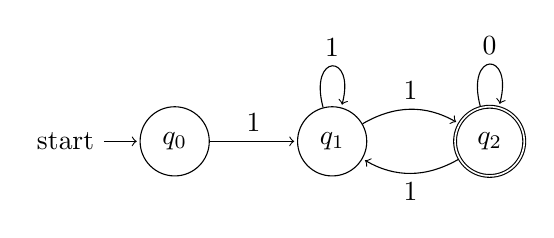
\begin{tikzpicture}[shorten >=1pt,node distance=2cm,on grid,auto] 
   \node[state,initial] (q_2)   {$q_0$}; 
   \node[state] (q_0)  [right=of q_2] {$q_1$}; 
   \node[state,accepting](q_1) [right=of q_0] {$q_2$};
    \path[->] 
    (q_0) edge [bend left]node {1} (q_1)
          edge [loop above] node {1} (q_0)
    (q_1) edge [bend left]node  {1} (q_0)
          edge [loop above] node {0} ()
    (q_2) edge node {1} (q_0);
\end{tikzpicture}


\subsubsection{b}
{w|w contains at least 3 1's}\\
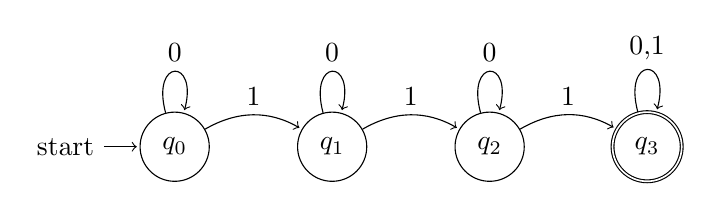
\begin{tikzpicture}[shorten >=1pt,node distance=2cm,on grid,auto] 
   \node[state,initial] (q_0)   {$q_0$}; 
   \node[state](q_1) [right=of q_0] {$q_1$};
   \node[state](q_2) [right=of q_1] {$q_2$};
   \node[state,accepting](q_3) [right=of q_2] {$q_3$};
    \path[->] 
    (q_0) edge [bend left]node {1} (q_1)
          edge [loop above] node {0} ()
    (q_1) edge [bend left]node  {1} (q_2)
          edge [loop above] node {0} ()
    (q_2) edge [bend left]node  {1} (q_3)
          edge [loop above] node {0} ()
    (q_3) edge [loop above] node {0,1} ();
\end{tikzpicture}


\subsubsection{c}
{w|w contains the substring 0101, (i.e. w = x0101y for some x and y)}
\\
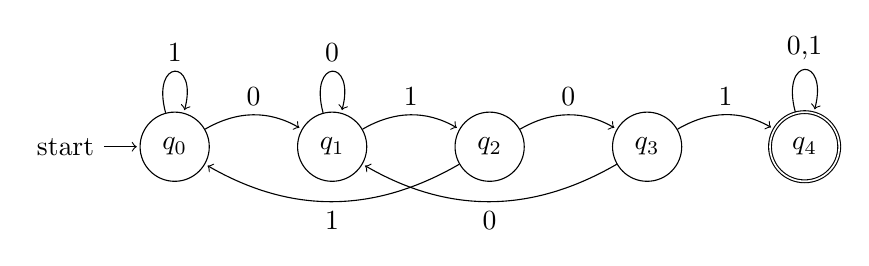
\begin{tikzpicture}[shorten >=1pt,node distance=2cm,on grid,auto] 
   \node[state,initial] (q_0)   {$q_0$}; 
   \node[state](q_1) [right=of q_0] {$q_1$};
   \node[state](q_2) [right=of q_1] {$q_2$};
   \node[state](q_3) [right=of q_2] {$q_3$};
      \node[state,accepting](q_4) [right=of q_3] {$q_4$};
    \path[->] 
    (q_0) edge [bend left]node {0} (q_1)
          edge [loop above] node {1} ()
          
    (q_1) edge [bend left]node  {1} (q_2)
          edge [loop above] node {0} ()
          
    (q_2) edge [bend left]node  {0} (q_3)
          edge [bend left] node {1} (q_0)
          
    (q_3) edge [bend left]node  {1} (q_4)
          edge [bend left] node {0} (q_1)
          
    (q_4) edge [loop above] node {0,1} ();
\end{tikzpicture}

\subsubsection{d}
{w|w bas at length of at least 3 and it's third symbol is 0}
\\
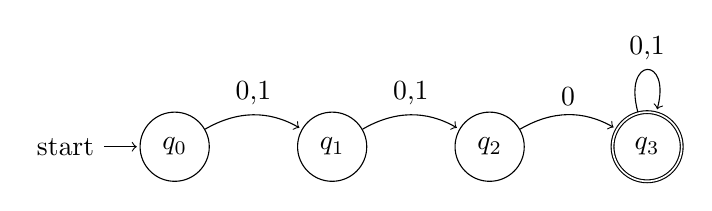
\begin{tikzpicture}[shorten >=1pt,node distance=2cm,on grid,auto] 
   \node[state,initial] (q_0)   {$q_0$}; 
   \node[state](q_1) [right=of q_0] {$q_1$};
   \node[state](q_2) [right=of q_1] {$q_2$};
   \node[state,accepting](q_3) [right=of q_2] {$q_3$};
    \path[->] 
    (q_0) edge [bend left]node {0,1} (q_1)
    (q_1) edge [bend left]node  {0,1} (q_2)
    (q_2) edge [bend left]node  {0} (q_3)
    (q_3) edge [loop above] node {0,1} ();
\end{tikzpicture}

\subsubsection{f}
{w|w doesn't contain the substring 001} \\
Accepts any string that doesn't contain the substring 001, and loops in rejecting state if this state is found, was unsure if the looping was needed but included it if it was the case.
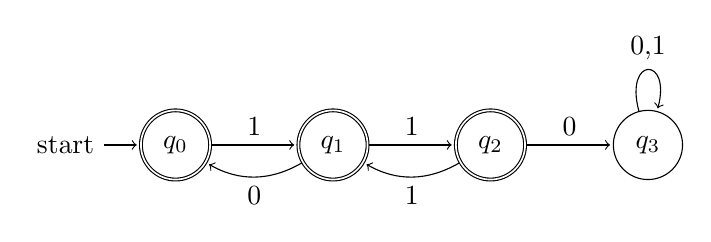
\begin{tikzpicture}[shorten >=1pt,node distance=2cm,on grid,auto] 
   \node[state,initial,accepting] (q_0)   {$q_0$}; 
   \node[state,accepting](q_1) [right=of q_0] {$q_1$};
   \node[state,accepting](q_2) [right=of q_1] {$q_2$};
   \node[state](q_3) [right=of q_2] {$q_3$};
    \path[->] 
    (q_0) edge node {1} (q_1)
    (q_1) edge node  {1} (q_2)
          edge [bend left] node {0} (q_0)
    (q_2) edge node  {0} (q_3)
    	edge [bend left] node {1} (q_1)
    (q_3) edge [loop above] node {0,1} ();
\end{tikzpicture}

\subsubsection{h}
{w|w is any string except 11 and 111}\\
accepts any string that isn't 11, 111 including the empty string $\epsilon $ \\
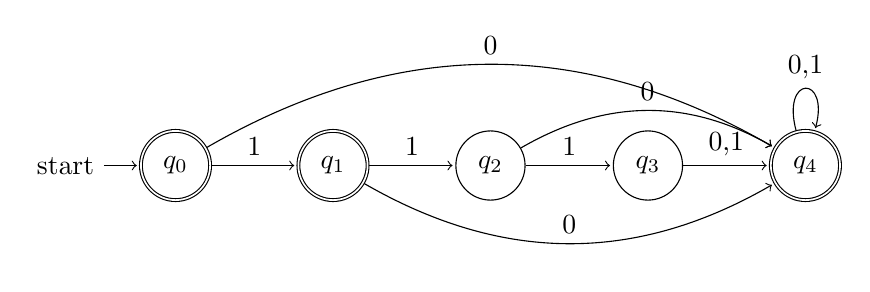
\begin{tikzpicture}[shorten >=1pt,node distance=2cm,on grid,auto] 
   \node[state,initial,accepting] (q_0)   {$q_0$}; 
   \node[state,accepting](q_1) [right=of q_0] {$q_1$};
   \node[state](q_2) [right=of q_1] {$q_2$};
   \node[state](q_3) [right=of q_2] {$q_3$};
   \node[state,accepting](q_4) [right=of q_3] {$q_4$};
    \path[->] 
    (q_0) edge node {1} (q_1)
   		  edge [bend left] node {0} (q_4)
    (q_1) edge node  {1} (q_2)
    	  edge [bend right] node {0} (q_4)
    (q_2) edge node  {1} (q_3)
    	  edge [bend left] node {0} (q_4)
    (q_3) edge node {0,1} (q_4)
    (q_4) edge [loop above] node {0,1} ();
\end{tikzpicture}

\subsubsection{i}
{w|w every odd position of w is a 1} \\
accepts all states where \#1\#1\#1\#1\#1 is followed also accepts the empty string $ \epsilon $ \\


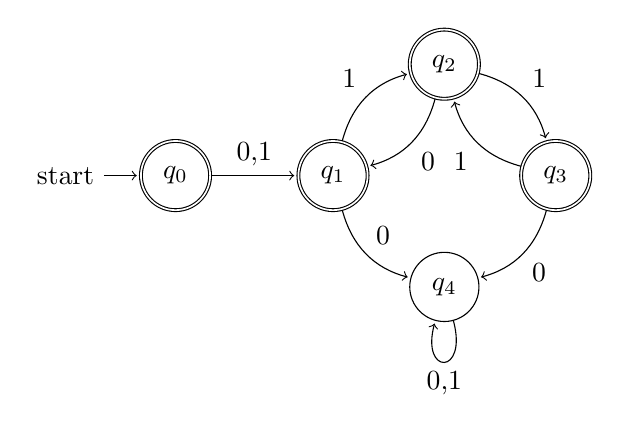
\begin{tikzpicture}[shorten >=1pt,node distance=2cm,on grid,auto] 
   \node[state,initial,accepting] (q_0)   {$q_0$}; 
   \node[state,accepting](q_1) [right=of q_0] {$q_1$};
   \node[state,accepting](q_2) [above right=of q_1] {$q_2$};
   \node[state](q_4) [below right=of q_1] {$q_4$};
   \node[state,accepting](q_3) [above right=of q_4] {$q_3$};
    \path[->] 
    (q_0) edge node {0,1} (q_1)
    (q_1) edge [bend left]node  {1} (q_2)
          edge [bend right] node {0} (q_4)
    (q_2) edge [bend left] node  {1} (q_3)
    	  edge [bend left] node {0} (q_1)
    (q_3) edge [bend left] node {0} (q_4)
   		  edge [bend left] node {1} (q_2)
   	(q_4) edge [loop below] node {0,1} ();
\end{tikzpicture}


\subsubsection{k}
{w|w is only the empty string and 0} \\
accepts "0" and the empty string $ \epsilon $ \\


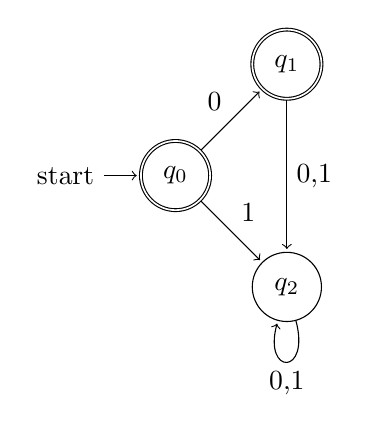
\begin{tikzpicture}[shorten >=1pt,node distance=2cm,on grid,auto] 
   \node[state,initial,accepting] (q_0)   {$q_0$}; 
   \node[state,accepting](q_1) [above right =of q_0] {$q_1$};
   \node[state](q_2) [below right =of q_0] {$q_2$};

    \path[->] 
    (q_0) edge node {0} (q_1)
    	  edge node  {1} (q_2)
    (q_1) edge node {0,1} (q_2)
   	(q_2) edge [loop below] node {0,1} ();
\end{tikzpicture}

\newpage
\subsection{page 84, question 1.7}

\subsubsection{d}
The language {0} with two states,\\

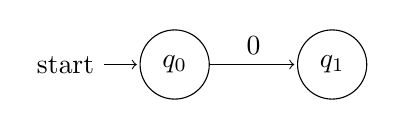
\begin{tikzpicture}[shorten >=1pt,node distance=2cm,on grid,auto] 
   \node[state,initial] (q_0)   {$q_0$}; 
   \node[state](q_1) [right =of q_0] {$q_1$};

    \path[->] 
    (q_0) edge node {0} (q_1);
\end{tikzpicture}
\subsubsection{e}
the language 0*1*0* with 3 states \\
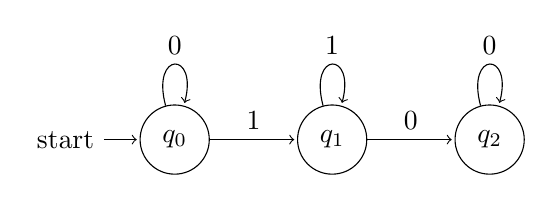
\begin{tikzpicture}[shorten >=1pt,node distance=2cm,on grid,auto] 
   \node[state,initial] (q_0)   {$q_0$}; 
   \node[state](q_1) [right =of q_0] {$q_1$};
   \node[state](q_2) [right =of q_1] {$q_2$};

    \path[->] 
    (q_0) edge node {1} (q_1)
    	edge [loop above]node  {0} (q_2)
    (q_1) edge node {0} (q_2)
    edge [loop above]node  {1} (q_2)
   	(q_2) edge [loop above]node  {0} (q_2);
\end{tikzpicture}
\subsubsection{g}
the language {$\epsilon$} with 1 state \\

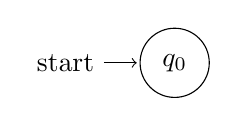
\begin{tikzpicture}[shorten >=1pt,node distance=2cm,on grid,auto] 
   \node[state,initial] (q_0)   {$q_0$}; 
\end{tikzpicture}


\subsubsection{h}
The language 0* with 1 state \\

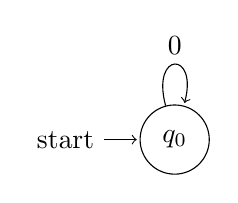
\begin{tikzpicture}[shorten >=1pt,node distance=2cm,on grid,auto] 
   \node[state,initial] (q_0)   {$q_0$}; ;

    \path[->] 
    (q_0) [loop above]edge node {0} ();
\end{tikzpicture}


\subsection{Solve the following problem,}

A man is travelling with a wolf (w) and a goat (g). He also brings along a nice big
cabbage (c). He encounters a small river which he must cross to continue his travel.
Fortunately, there is a small boat at the shore which he can use. However, the boat
is so small that the man cannot bring more than himself and exactly one more item
along (from {w, g, c}). The man knows that if left alone with the goat, the wolf will
surely eat it and the goat if left alone with the cabbage will also surely eat that. The
man’s task is hence to device a transportation scheme in which, at any time, at most
one item from {w, g, c} is in the boat and the result is that they all crossed the river
and can continue unharmed.

\subsubsection{a} Describe a solution to the problem which satisfies the rules of the “game”. You may use your answer to (b) to find a solution. \\

\begin{itemize}
\item First you carry the goat to the other side, and go back empty.
\item The you ferry the wolf to the other side, and swap with the goat and bring the goat back.
\item you then swap the goat with the cabbage and bring it to the other side.
\item lastly you head back empty and bring the goat.
\item you now have all the items on the other side of the river.
\end{itemize}


\subsubsection{b}
The string all of the valid moves are 
\begin{equation}
\begin{split}
(g(m(x(g(y(m(g)*)*)*)*)*)*)* \\
x,y = (w|c) \\
x \neq y
\end{split}
\end{equation}


\vspace{5mm}
This is due to the fact that it's legal moves in the game, like the man can bring the goat to the other side and bring it back too, it's bad move, but it's still a valid move. \\

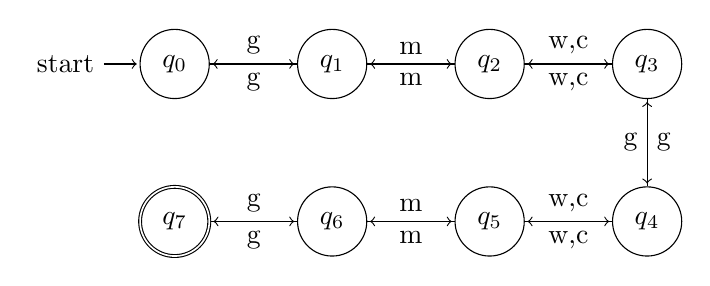
\begin{tikzpicture}[shorten >=1pt,node distance=2cm,on grid,auto] 
   \node[state,initial] (q_0)   {$q_0$}; 
   \node[state](q_1) [right =of q_0] {$q_1$};
   \node[state](q_2) [right =of q_1] {$q_2$};
   \node[state](q_3) [right =of q_2] {$q_3$};
   \node[state](q_4) [below =of q_3] {$q_4$};
   \node[state](q_5) [left =of q_4] {$q_5$};
   \node[state](q_6) [left =of q_5] {$q_6$};
   \node[state,accepting](q_7) [left =of q_6] {$q_7$};

    \path[->] 
    (q_0) edge node {g} (q_1)
    (q_1) edge node {g} (q_0)
   	      edge node {m} (q_2)
    (q_2) edge node {m} (q_1)
   	      edge node {w,c} (q_3)
   	(q_3) edge node {w,c} (q_2)
   	      edge node {g} (q_4)
   	(q_4) edge node {g} (q_3)
   	      edge node {w,c} (q_5)
   	(q_5) edge node {w,c} (q_4)
   	      edge node {m} (q_6)
   	(q_6) edge node {m} (q_5)
   	      edge node {g} (q_7)   	      
   	(q_7) edge node {g} (q_6);
\end{tikzpicture}




\section{Week 2}

\subsection{page 86, question 1.16}
* is any number \\
! is one or more \\

\subsubsection{a}
it accepts (bb)*a!(a|b)* \\

the language 0*1*0* with 3 states \\
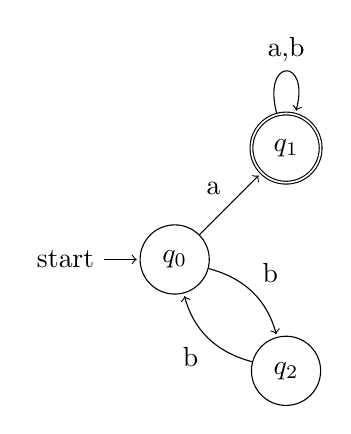
\begin{tikzpicture}[shorten >=1pt,node distance=2cm,on grid,auto] 
   \node[state,initial] (q_0)   {$q_0$}; 
   \node[state,accepting](q_1) [above right =of q_0] {$q_1$};
   \node[state](q_2) [below right =of q_0] {$q_2$};

    \path[->] 
    (q_0) edge node {a} (q_1)
   		  edge [bend left]node {b} (q_2)
    (q_1) edge [loop above]node {a,b} (q_1)
   	(q_2) edge [bend left]node  {b} (q_0);
\end{tikzpicture}

\subsubsection{b}


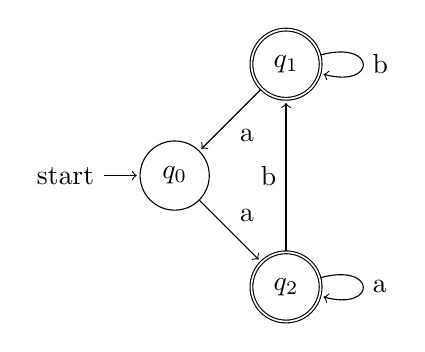
\begin{tikzpicture}[shorten >=1pt,node distance=2cm,on grid,auto] 
   \node[state,initial] (q_0)   {$q_0$}; 
   \node[state,accepting](q_1) [above right =of q_0] {$q_1$};
   \node[state,accepting](q_2) [below right =of q_0] {$q_2$};

    \path[->] 
    (q_0) edge node {a} (q_2)
   		  
    (q_1) edge node {a} (q_0)
    	  edge [loop right]node {b} ()
   	(q_2) edge [loop right]node  {a} ()
   	      edge []node  {b} (q_1);
\end{tikzpicture}

\subsection{page 86, question 1.17}

\subsubsection{a}
The first task is to make a NFA recognizing (01u001u010)* \\
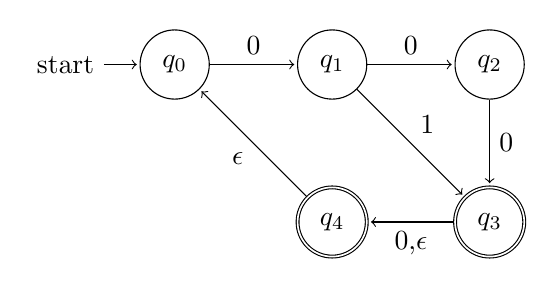
\begin{tikzpicture}[shorten >=1pt,node distance=2cm,on grid,auto] 
   \node[state,initial] (q_0)   {$q_0$}; 
   \node[state](q_1) [right =of q_0] {$q_1$};
   \node[state](q_2) [right =of q_1] {$q_2$};
   \node[state,accepting](q_3) [below =of q_2] {$q_3$};
   \node[state,accepting](q_4) [below =of q_1] {$q_4$};



    \path[->] 
    (q_0) edge node {0} (q_1)
    (q_1) edge node {0} (q_2)
    	  edge node {1} (q_3)
   	(q_2) edge node {0} (q_3)
   	(q_3) edge node {0,$\epsilon$} (q_4)
   	(q_4) edge node {$\epsilon$} (q_0);
\end{tikzpicture}
\\

\subsubsection{b}
After converting this to a DFA\\

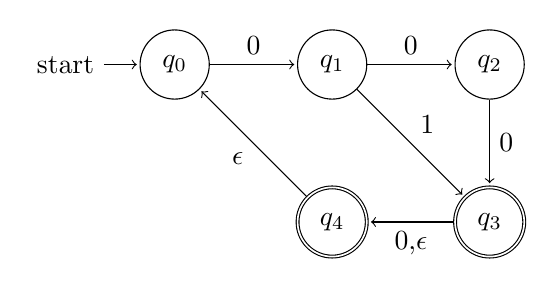
\begin{tikzpicture}[shorten >=1pt,node distance=2cm,on grid,auto] 
   \node[state,initial] (q_0)   {$q_0$}; 
   \node[state](q_1) [right =of q_0] {$q_1$};
   \node[state](q_2) [right =of q_1] {$q_2$};
   \node[state,accepting](q_3) [below =of q_2] {$q_3$};
   \node[state,accepting](q_4) [below =of q_1] {$q_4$};



    \path[->] 
    (q_0) edge node {0} (q_1)
    (q_1) edge node {0} (q_2)
    	  edge node {1} (q_3)
   	(q_2) edge node {0} (q_3)
   	(q_3) edge node {0,$\epsilon$} (q_4)
   	(q_4) edge node {$\epsilon$} (q_0);
\end{tikzpicture}

\subsection{page 86, question 1.18}
Predefined terms
\begin{equation}
x = (0,1)^*
\end{equation}
\begin{equation}
y = (0|1)
\end{equation}

\subsubsection{a}
$1x0$
\subsubsection{b}
$x1x1x1x$
\subsubsection{c}
$x0101x$
\subsubsection{d}
$yy0x$
\subsubsection{e}
$(0(yy)*)|1y(yy)^*)$
\subsubsection{f}
$ 0^*(1+10)^* $
\subsubsection{g}
$ yyyyy $


\subsection{page 86, question 1.19 a}

Convert the following regex to a NFA via lemma 1.55\\
\begin{equation}
(0 \cup 1)^*000(0\cup 1)^* 
\end{equation}
\begin{center}


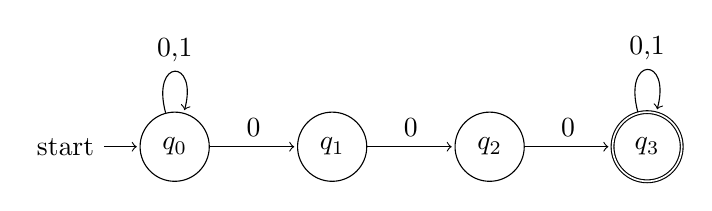
\begin{tikzpicture}[shorten >=1pt,node distance=2cm,on grid,auto] 
   \node[state,initial] (q_0)   {$q_0$}; 
   \node[state](q_1) [right =of q_0] {$q_1$};
   \node[state](q_2) [right =of q_1] {$q_2$};
   \node[state,accepting](q_3) [right =of q_2] {$q_3$};



    \path[->] 
    (q_0) edge [loop above] node {0,1} (q_0)
    	  edge node {0} (q_1)
    (q_1) edge node {0} (q_2)
   	(q_2) edge node {0} (q_3)
   	(q_3) edge [loop above] node {0,1} ();
\end{tikzpicture}
\end{center}

\subsection{page 86, question 1.20}
\subsubsection{a}
\begin{equation}
a^*b^*
\end{equation}
member
aa, ab, aabb, aab, abbbb
not member
ba, abab, 
\subsubsection{b}
member
abab, ababababab,
not member
aaba baba
\subsubsection{c}
member
ab, aabb,
not memeber
ba, aabba
\subsubsection{d}
member
aaa, aaaaaa
not memeber
a, aaaa
\subsubsection{e}
member

not memeber
\subsubsection{f}
member

not memeber
\subsubsection{g}
member
ab, b
not memeber
abb, aab
\subsubsection{h}
member

not memeber

\subsection{page 86, question 1.21 b}

The solution is 
\begin{equation}
((a|b)(a,bb)*b(a)?)*
\end{equation}
(a or b, followed by any number of (a,bb)* followed by a single b (as it matches uneven numbers of b and followed by 0 or 1 a*

\subsection{page 86, question 1.29}

\subsubsection{a}

For the task a we have the sting 
\begin{equation}
0^n1^n2^n
\end{equation}
the first contradiction is that when we have a string eg. 000111222 and we split it so we have the floowing, x = 000, y = 111, z = 222 and we pump y so we have the string xyyz this violates the first condition of the pumping lemma, as we'll have more 1s then 0s and 2s.

the string y only contains 1s which also causes a contradiction.

and the 3rd case if we have the string x = 00, y = 011 and z = 1222 where we'll get out of order letters so we'll again reach a contradiction.


\subsubsection{b}

For assignment b i find it a bit odd, i may misunderstand the exercise but w/e

We want to pump the language
\begin{equation}
a_2 = \{www|w \in \{a,b\}^*\}
\end{equation}
But from my understanding is the * a klein star? eg then one w and www are equivalent as \{a,b\} is all possibly strings in the library w. ? or is it understand such that w is equal to either a or b but any number of them eq $\{a|b\}^*$,\\
How i choose to intercept it for now is that w is equal to either the string a* or b* and if this is the case then some of the same argumentation as for task a is valid.
\\
www can give us the string 111000111 and we can split it as follows. 111|1000|11111, This means that zyyx gives of a out of order 1 and we therefor get a contradiction wrt. to the pumping lemma.






\newpage
\chapter{Questions 2018}
\newpage
\section{1. Finite automata and regular languages}

Introduction
What is it

	Finite automata, regular languages
	
regular languages
aboveabove
Finite atomata

Nondetermanistic


NFA
DFA


Pumping lemma for regular languages






\newpage
\section{2. Pushdown automata and context-free languages}

%Chomsky normal form.


What is a push down

What is a context free grammar
a -> 0a1
A -> B
B -> \#
    ambiguity
    grammar
    variables


What can it be used to
    programming languages
    Compiler
    
    

        
Pushdown atomata in dept
    You use a stack.
    
Pumping lemma
    Proof
    
    Application
    



\newpage
\section{3. Turing machines}

Introduction
    What is a turning machine
        
Multitape

Nondetermanistic turning machine
    Faster but less powerfull?
    



\newpage
\section{4. Decidability}
Introduction
 If a language  defined by a DFA is decidable.


Examples of Decidability and undecidability




\newpage
\section{5. Reducibility}
What is it and how to use it.





\newpage
\section{6. NP-completeness proofs – examples.}
what is np\_completeness

Why we use it to reduce,

Proff of np complete.
qlique, subset sum, Hamiltonian circuit, 




\newpage
\section{7. Proof that SATISFIABILITY is NP-complete (do not assume that
there is a known NP-Complete problem — use the proof in Sipser’s
book).}

Cook-levin theorem - insipset, præsentation use slides on homepage.
\newpage
\section{8. Information-theoretic lower bounds (lower bounds proven by counting
leaves in decision trees), especially the average case bounds for sorting
by comparisons.}
As is average case.




\newpage
\section{9. Adversary arguments – technique, examples.}





\newpage
\section{10. Median problem – algorithm and lower bound.}





\newpage
\section{11. Approximation algorithms}













%%%%%%%%%%%%%%%%%%%%%%%%%%%%%%%%%%%5
\newpage
\chapter{Questions 2017}
\section{Questions from last year}
1. Finite automata and regular languages \\
2. Pushdown automata and context-free languages\\
3. Turing machines\\
4. Decidability\\
5. Reducibility\\
6. NP-completeness proofs – examples.\\
7. Proof that SATISFIABILITY is NP-complete.\\
8. Information-theoretic lower bounds (lower bounds proven by counting leaves in decision trees), especially the average case bounds for  sorting by comparisons.\\
9. Adversary arguments – technique, examples.\\
10. Approximation algorithms.\\
\newpage
\subsection{1. Finite automata and regular languages}
\subsubsection{Introduction}
\subsubsection{Types of Automata}
	DFA - 
    NDFA - 

\newpage
\subsection{2. Pushdown automata and context-free languages}
	CFG(context free grammar)
    	regular language
        	defined by DFA
           ambiguity
           		inherited ambiguity
           Chomsky normal form
           		You're allowed to have a rule that turns A into two sub rules.
           			A -> BC
                You can have a rule about a terminal set for our alphabet.
                	$A -> a \in \sum \epsilon $
                You're only allowed to produce Epsilon from the start symbol.
                	$S -> \epsilon $
            theorem
            	Any CFL is generated by a CFG in Chomsky normal form,
                
    pushdown automata PDA(s) 
    		NFA with a stack.
    	
    	
           
\subsection{3. Turing machines}
\subsection{4. Decidability}
\subsection{5. Reducibility}
\subsection{6. NP-completeness proofs – examples.}
\subsection{7. Proof that SATISFIABILITY is NP-complete.}
\subsection{8. Information-theoretic lower bounds (lower bounds proven by counting leaves in decision trees), especially the average case bounds for sorting by comparisons.}
\subsection{9. Adversary arguments – technique, examples.}
\subsection{10. Approximation algorithms}

\newpage
\chapter{Lectures}
\subsection{Format}
Titles should be listed as (date - topic(s)) for easier lookup

\subsection{28-feb-2018 - TBD}
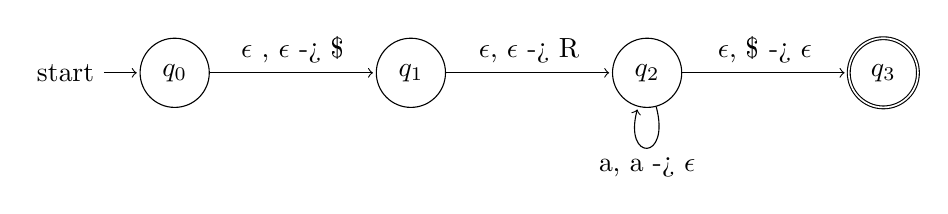
\begin{tikzpicture}[shorten >=1pt,node distance=3cm,on grid,auto] 
   \node[state,initial] (q_0)   {$q_0$}; 
   \node[state] (q_1) [right=of q_0] {$q_1$}; 
   \node[state] (q_2) [right=of q_1] {$q_2$}; 
   \node[state,accepting](q_3) [right=of q_2] {$q_3$};
    \path[->] 
    (q_0) edge  node {$\epsilon$ , $\epsilon$ -> \$} (q_1)
    (q_1) edge  node {$\epsilon$, $\epsilon$ -> R} (q_2)
    (q_2) edge  node {$\epsilon $, \$ -> $ \epsilon $} (q_3) 
          edge [loop below] node {
          a, a -> $\epsilon$} (); 
\end{tikzpicture}


\section{22 march }
\subsection{assignment 2}
We can reconnize that it is two regular languages, and that when we concatinate them we get a reglang\\
sigma star is regular, \\
we can apply theom 1.49 regular langs are closed under concat.\\
\subsection{assignemnt 3}


d)\\
	use p from pumping lemma \\
    $(xy)^{3p}(x)^p$ \\
     q

\subsection{assignemnt 5}
a)
	prove by counter exsample
    \\
    ${a^ib^ic^i | i \geq 0} \cup {a,b,c}^* $
b)
	prove by counter exsample
	${a^ib^ic^i | i \geq 0} \cup {\emptyset}$
    
    


\section{10th of April}
\begin{itemize}
\item Polynomial time reductions
\item NP-completeness
\item Examples of proofs
\begin{itemize}
\item 3-SAT
\item CLIQUE
\item Vertex cover
\item Independent set
\end{itemize}
\end{itemize}


\newpage
\section{12th of April}
\subsection{CNE-SAT is NP-Complete}
\subsubsection{Cook-lenin thm}
SAT is NP-Complete\\
 	Show that:\\
    \begin{equation}
    \forall A \in NP : A \leq_p SAT,
    \end{equation}
$ A \in NP $, Let N be a polytime NTM which accepts it in time $d_1n^k +d_2$ \\
\begin{equation}
N = (Q,\sum,R, \alpha, q_o, q_accept, q_reject).
\end{equation}
Let $W = W_1W_z*W_n$ be input to A,\\
Crate (in  polytime) a boolean formula F which is satisfiable if W is accepted by N,\\
Look at accepting breach of computation tree\\
Look at sequence of configurations.
    
\subsection{Subset-sum is NP-Complete}
   
\section{17th of April}
Hamiltonian circuit is NP-complete
\\
Conclusion on NP-complete
\\
Information on theoretic lower bound technique.

\section{1st of may}
    Approximation algorithms
    \\
    $\delta$-TSP has 2-approximation algs
    \\
    For general TSP and a fixed P, $\Delta $an alg with approx p
    \\
    Vertex cover has a 2-approx alg.
 
\end{document}

